\documentclass[sigconf]{acmart}
\usepackage{threeparttable}
\usepackage{booktabs} % For formal tables
\settopmatter{printacmref=false} % Removes citation information below abstract
\renewcommand\footnotetextcopyrightpermission[1]{} % removes footnote with conference information in first column
\pagestyle{plain} 

% Copyright
%\setcopyright{none}
%\setcopyright{acmcopyright}
%\setcopyright{acmlicensed}
\setcopyright{rightsretained}
%\setcopyright{usgov}
%\setcopyright{usgovmixed}
%\setcopyright{cagov}
%\setcopyright{cagovmixed}



\acmArticle{4}
\acmPrice{15.00}

% These commands are optional
%\acmBooktitle{Transactions of the ACM Woodstock conference}
\editor{Yifei Wu}


\begin{document}

\begin{center}
UNIVERSITY OF CALIFORNIA\\
\ \\
SANTA CRUZ\\
\ \\
{\bf A STORY RECOMMENDATION SYSTEM FOR A KIDS CHATBOT, SLUGCHAT}\\
\ \\
A report submitted in partial satisfaction\\
of the requirements for the degree of\\
\ \\
MASTER OF SCIENCE\\
\ \\
in\\
\ \\
COMPUTER SCIENCE\\
\ \\
by\\
\ \\
{\bf Yifei Wu}\\
\ \\
December 2017\\
\ \\
\ \\
\ \\
\end{center}

{\addtolength{\leftskip}{120 mm}
\ \\
The Report of Yifei Wu \\
is approved:\\
\ \\
\ \\
--------------------------------------------------\\
Professor Yi Zhang, Chair\\
\ \\
\ \\
--------------------------------------------------\\
Professor Luca de Alfaro\\

}
\ \\
\ \\
\ \\
\ \\
--------------------------------------------------\\
Tyrus Miller\\
Vice Provost and Dean of Graduate Studies

\pagebreak[4]


\title{A Story Recommendation System for a Kids Chatbot,  SlugChat}


\author{Yifei Wu}
\affiliation{\institution{University of California, Santa Cruz}}
\email{ywu151@ucsc.edu}


% The default list of authors is too long for headers.
\renewcommand{\shortauthors}{B. Trovato et al.}


\begin{abstract}
Listening and speaking are important skills for kids. They improve kids' intelligence and verbal ability. The booming of AI chatbot technology provides a good method for kids to practice these skills. With the increasing time children spending on smart devices, there is a growing interest in mobile chatbots for kids. In this paper, we propose a story recommendation system deployed on a kids mobile chatbot, SlugChat. The proposed system collects stories and their listening behaviors. It get preferences by using story vectors to train LSTM model. We also propose how we deploy this system to the chatbot.
\end{abstract}

\maketitle

%----------------------------------------------------------------------------------------
%	ARTICLE CONTENTS
%----------------------------------------------------------------------------------------

\section{Introduction}
Childhood is the beginning of human life and plays an essential role. Some researchers show that a better childhood may provide a better development in many fields like intelligence and verbal ability. A good method to achieve these is talking more with kids especially in their first eight years\cite{happe1995role,jones1972home}.
\\\\
Most children could get a better vocabulary acquisition by listening to stories and explanations of target words from their parents\cite{brett1996vocabulary}. However, not all parents have enough time to chat with their kids. For example, a report indicts that over 90\% children complain their parents lack of time to chat with\cite{wccd}.
\\\\
On the other hand, although some parents would not have enough time to speak to their kids, children spend increasing time on electronic devices\cite{vandewater2007digital}. These devices use many technologies to improve user experience, such as AI chatbot and recommendation system.
\\\\
AI chatbot offers children an excellent platform to practise verbal ability. Furthermore, recent reports show that kids under 6 have great interests in interacting with electronic devices despite limited literacy\cite{as}. Nowadays, almost all IT giants develop their own chatbot like Amazon's Alexa which provides functions over Music \& Radio, Game or Trivia, and Podcast\cite{rh}. Among these chatbot, there are also excellent products for kids, such as Tyche, ibotn, BeanQ, and Apphome\cite{cb}.
\\\\
Recommendation systems have the effect of guiding users in a personalized way to interesting objects in a large space of possible options\cite{lops2011content}. In today's world, recommendation systems have become more and more popular. Some recommendation algorithms are based on users' behaviors\cite{liu2010personalized}. Songs, movies, news and so many things could be recommended to users based on their and others' previous behaviors. It not only saves time but also encourages people to generate more behaviors. Then algorithms would recommend more right things to users.
Unfortunately, most of current recommendation systems are for all ages. And there are no public available papers about recommendation systems about children's literacy, such as short stories for kids.
\\\\
In this paper, we present a short story recommendation system in Mandarin for kids between three to six years old. We deploy this system on a new mobile application for kids, Slugchat, who has the abilities to tell stories, sing children's songs, read poems, and answer some general questions for kids.

%------------------------------------------------

\section{Related Work}
In order to build a story recommendation system and deploy it on a chatbot, we need technologies from different areas. We introduce these technologies in this section.

\subsection{Web Crawler}
A web crawler, sometimes called a spider, is a program which is able to browse the World Wide Web methodically and automatically\cite{dhenakaran2011web}. A web crawler collects massive data from various sources. This data remains in an unstructured form. We call them raw data and we need to derive useful values from them. Thus, a web crawling is usually the first step of many work.

\subsection{Word Segmentation}
In languages such as English, words are separated by spaces. While there are no spaces beween words in sentences in Mandarin. It is hard to analysis word token directly. In this project, we use a python liberary $jieba$ to do word segmentation. We build a  dictionary for kids. 

\subsection{Word Vector}
Word2vec is a group of related models. Each unique word is assigned a vector in a space (or location). Words contain familiar contexts are located nearby\cite{goldberg2014word2vec}. These models could be trained by giving a large corpus of text. In this project, we build word2vec models for kids' words in Mandarin.

\subsection{Story Vector}
There are several ways to represent a story, such as Word Mover's Distance\cite{kusner2015word}, Bag of Words and Paragraph Vector\cite{le2014distributed}. In this project, we use Bag of Words to represent stories. And in future work, we will use the states in RNN to present each story.

\subsection{Recommendation System}
Recommendation systems filter useful information to predict the preference of a user by giving items\cite{ricci2011introduction, grossman2010computers}. Generally, there are two kinds of recommendation algorithms, collaborative filtering and content-based\cite{jafarkarimi2012naive}.  Collaborative filtering algorithms are based on users' data, such as behaviors, activities and preferences. They predict the results based on not only the user's own data but also data from similar users\cite{breese1998empirical}. Content-based filtering algorithms predict the relation between features or labels of items and preferences of users\cite{aggarwal2016recommender}. While, it is also feasible to combine these two kinds of algorithms in order to predict more accurately and effectively. They are hybrid recommendation systems/cite{adomavicius2005toward}.
In this project, we develop a story recommendation system based on children's listening behaviors.

\subsection{Dialogue System}
The developers of dialogue systems need to design conversation flows and rules to make systems work well\cite{abdul2015survey}. Luckily, there are some wonderful platforms, such as Dialogflow, wit.ai, IBM Watson, Microsoft LUIS and Rulai. They help developers build systems automatically and provide codeless interfaces for designing dialogue flows\cite{mctear2016introducing}. In this project, we use to Dialogflow. We build a set of intents, entities and contexts to implement our dialogue and we use webhook to post responses to our servers.

\section{Project Design}
In this section, we show how we design our project. For each step, we list all possible methods, compare their practicalities and performances and choose the suitable one.

\subsection{Data Collection}
The first step to build this recommendation system is collecting suitable stories for kids. We can not just download the text set of stories from the Internet directly because of the following reasons:
\begin{enumerate}
\item Our users are kids between three to six years old. Parts of them may have limited literacy. Thus, we need to provide stories with audios.
\item Our recommendation algorithm is based on the content of stories. Thus, our stories should also have text. 
\item For the cold start, we need to know the styles and target ages for each story.
\end{enumerate}
In summary, we need stories with exactly the same text and auto type, target ages, styles and in Mandarin. After searching, we decided to use stories from a 
no copyright restrictions story website, Beva. We collect 700 stories in Beva.
\\\\
The second step is collecting the listening behaviors of our stories. There are four ways: collecting real users' listening behaviors through our chatbot, simulation kids' listening behaviors, searching existing data and crawling real data from the Internet. However, we only have 2 months to finish this project, there is not enough time for us to collect data by ourselves. Simulated data are lack of convincing and do not contain the implied relation among stories. And as described in Chapter 1, there is no story recommendation system for kids. Thus, the only way for us is crawling data from other websites.
\\\\
We collect the comments and their usernames under each story in Beva. Then we order stories with comments in time order for each username to get their listening lists. However, there are only 23 users who have listened to more than one story. And these users only listen to 54 stories among 700 stories. This data set is too small.
\\\\
Then, we crawl data from NetEase Cloud Music, which is a music and video streaming service website. There are stories for kids. And users are able to create their own playlists and share with others without copyright restrictions. The playlists are also listening lists of users. In this website, I collect 48908 listening lists. Their lengths distribution is shown in Figure \ref{fig:dlll}. This dataset is enough to be training data.

\begin{figure}
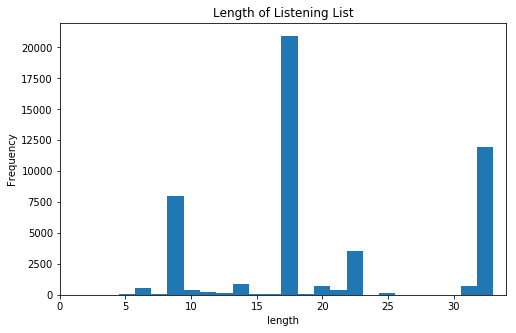
\includegraphics[width = .45\textwidth]{distribution_of_listening_list_length.png}
\caption{Distribution of Listening List Length}
\label{fig:dlll}
\end{figure}

\subsection{Data Preprocessing}
After getting stories and listening lists. We abstract words and stories to vectors.
\\\\
For word vectors, we use word2vec to build Chinese words models for kids. However, we only have 700 short stories whose text size is about 1.5 MB. This dataset can not provide enough implied information to train good word2vec models. After training, the average similarity between each two words is about 90\% which is horrible. The distribution of top 150 most frequent words in two-dimensional space is shown in Figure \ref{fig:word2vec_1_100}.
\\\\
Then we try to use pre-trained models in Chinese. And using principal component analysis to reduce the size of dimensions. We download several models including official Chinese model from Google and customized models which training from over 150 GB corpus. However, the Chinese language does have the similar concept as lemma and stem. It is hard to train a dictionary model which contains all Chinese words. In particular, our target users are kids, which means there are a few words are unusual. These pre-trained models fail in covering all words we need. We decided to enlarge our text corpus. We only need the suitable sentences for kids and do not need to find the same audio. Thus, we collect 24 MB children stories as our new text corpus. After training, we get acceptable Chinese word2vec models.
\\\\
For story vectors, we use Bag of Words first and evaluate its performance. In the future, we will use better models to improve this part.

\subsection{Recommendation Algorithm}
There are many recommendation algorithms. For example, matrix factorization without any content features is a classic collaborative filtering method. However, we can not use it. Our listening lists fail in covering all 700 stories. Even them could, our dataset will continually add new stories. 
Thus, we use Recurrent Neural Network (RNN) to extract content features in listening lists.
\\\\
There are two methods to build Recurrent Neural Network for our system.
\begin{enumerate}
\item Use each story vector as each input, as shown in Figure \ref{fig:rnn_story}. Story$_i$ is the \emph{i}th story vector in a listening list. 
\item Build a two-level neural network. Use each word vector in each sentence in each story as an input of the first level. Using the states of each story in the first level as the inputs of the second level, as shown in Figure \ref{fig:rnn_word}. X$_i$ is the list of word vectors of the \emph{i}th story in a listening list. 
\end{enumerate}
In this project, we realize the first method and evaluate its performance. In future work, we will realize other methods.

\begin{figure}
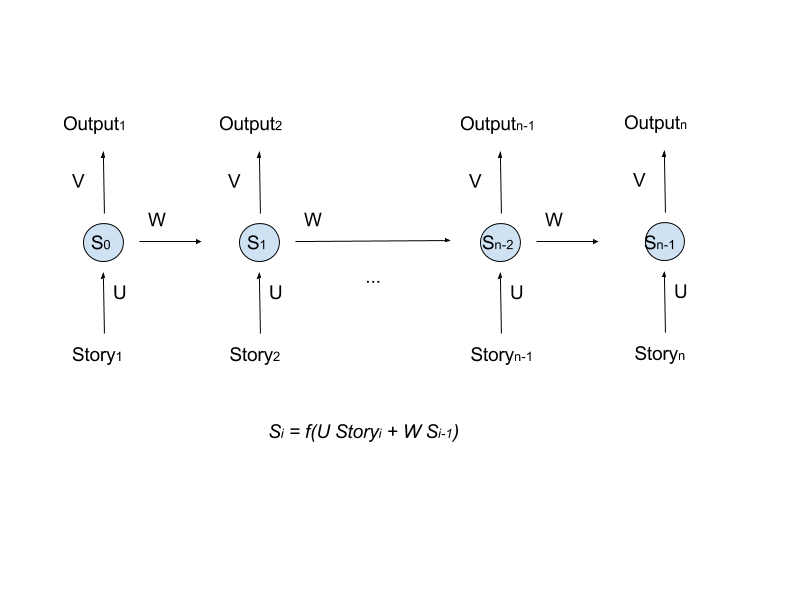
\includegraphics[width = .45\textwidth]{rnn_story.png}
\caption{RNN Story Vector}
\label{fig:rnn_story}

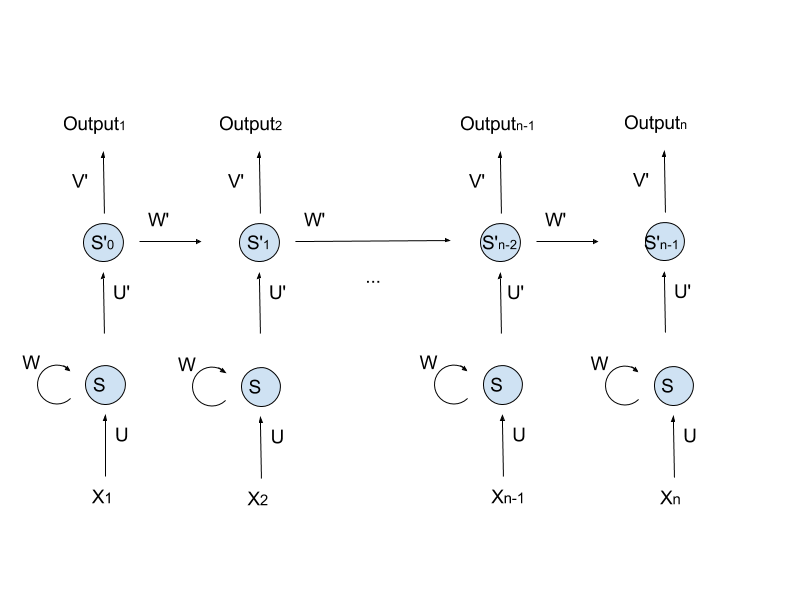
\includegraphics[width = .45\textwidth]{rnn_word.png}
\caption{RNN Word Vector}
\label{fig:rnn_word}
\end{figure}

\subsection{Dialogue Server}
We develop a mobile application, SlugChat. Its diagram is shown in Figure \ref{fig:diagram_slugchat}. It is able to talk with users (most of them are children). It has the following functions:
\begin{enumerate}
\item Answer general questions, such as \emph{'What is Beijing?'} and \emph{'Who is Washington?'}. 
\item Own human features like age, name. Users can interact with SlugChat about these.
\item Ask questions to users, such as  \emph{'Is there any interesting thing today?'}.
\item Reading poems based on users' words.
\item Reading stories to users.
\item Allow users to interrupt at any time. 
\end{enumerate}
In this project, we only focus on the backend of reading stories function. We need finish the following work:
\begin{enumerate}
\item Deploy an Amazon Relational Database Service. Create a story table to store stories and a log table to store users behaviors.
\item Deploy an Amazon Elastic Compute Cloud platform and build a backend server by express on it. This server has three post responses. Send a recommended story, send a story by its id and send a story by its title.  
\item Use Dialogflow to create story intents corresponding to the above post responses.
\end{enumerate}

\begin{figure}
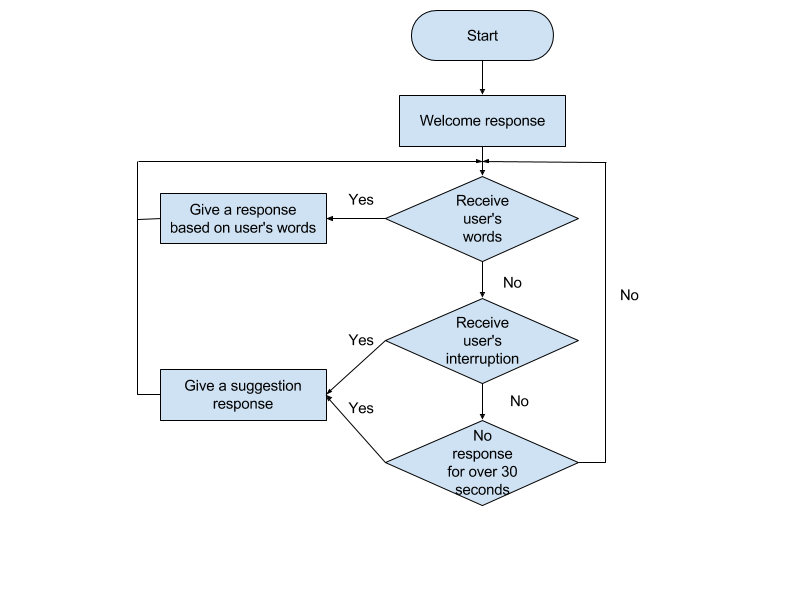
\includegraphics[width = .55\textwidth]{diagram_slugchat.png}
\caption{The Diagram of SlugChat}
\label{fig:diagram_slugchat}
\end{figure}

\section{Implementation}
In this section, we introduce the detailed steps about how to implement the whole project in each part.

\subsection{Data Collection}
Frist step is crawling stories, their feature and comments from Beva.
\begin{enumerate}
\item Get source code of each page for the story list for each age from 3 to 6 by python lib \emph{requests}.  
\item Get story divs by python lib \emph{bs4.BeautifulSoup}.
\item Extract story titles and content URLs from story divs.
\item Get the source code in story content page by URL.
\item Extract the content, style, audio link and get the request URL for comments by python lib \emph{re}.
\item Send a get request to get comment list.
\item Store stories and usernames of comments.
\item Store stories to database.
\end{enumerate}
The style and age distribution of stories are shown in Table \ref{tab:style_age_d}.
\\
\begin{table}
  \caption{Story Style and Age Distribution}
  \label{tab:style_age_d}
  \begin{threeparttable}
  \begin{tabular}{c|ccccc}
    \toprule
    Style & Total & Age3 & Age4 & Age5 & Age6\\
    \midrule
    Aesop's Fable & 147 & 67 & 76 & 99 & 133 \\
	Celebrity Story & 84 & 27 & 32 & 54 & 78 \\
	Andersen's Fairy & 20 & 18 & 18 & 18 & 18 \\
	Idiom Story  & 114 & 33 & 45 & 84 & 105 \\
	Grimm's Fairy & 77 & 47 & 60 & 66 & 63 \\
	Bedtime Story & 197 & 160 & 141 & 99 & 70 \\
	Fairy Tale & 61 & 51 & 56 & 55 & 47 \\
  \bottomrule
\end{tabular}
\begin{tablenotes}
        \footnotesize
        \item[1] Age\emph{i} means stories suitable for i-year-old kids.
        \item[2] Some stores are suitable for multiple ages.
      \end{tablenotes}
  \end{threeparttable}
\end{table}
\\
The second step is crawling listening behaviors from NetEase Cloud Music. Here are the detailed steps:
\begin{enumerate}
\item Get all story titles and remain all Chinese characters by \emph{re}.
\item Dynamically search \emph{'children story'} in playlist part in NetEase website by python lib \emph{selenium.webdriver}.
\item Extract URLs of playlists by \emph{BeautifulSoup} and add these URLs into a playlist queue $Q$.
\item Get story title list in the first playlist in queue $Q$ by $requests$ and remove this list from queue $Q$.
\item Remain the same stories in our story set.
\item If this playlist has the same stories in our story set, get the URLs of its preference playlists and add them into queue $Q$ if they are never added into queue $Q$ before.
\item Continue to next playlist in queue $Q$ until queue $Q$ is empty.
\end{enumerate}

\subsection{Data Preprocessing}
Frist step is training word2vec models.
\begin{enumerate}
\item Filtrate Chinese characters and stop punctuations of sentences from corpus by \emph{re}.
\item Split word tokens by python lib \emph{jieba}.
\item Remove stop words.
\item Store word tokens into a two-dimensional array. First dimension store sentence words and the second dimension story words.
\item Calculate word frequencies and rank words by frequencies.
\item Train word2vec models by python lib \emph{gensim}.
\item Reduce the number of dimension by python lib \emph{TSNE} and visualize these models by python lib \emph{matplotlib}
\item Evaluate the performance of these models.
\end{enumerate}
As described in Chapter 3.2, the first time we use text corpus with 700 stories and get bad models. The distribution of top 150 most frequent words in 2 dimensional space is shown in Figure \ref{fig:word2vec_1_100}.
\\\\
In order to get acceptable word2vec models, we crawl 24 MB story text file from many Chinese children story websites. Then we use this corpus to train word2vec models. We train different models with different vector sizes from 25 to 100. Finally, we choose to use models with vector size 50. The distribution of top 150 most frequent words in 2 dimensional space is shown in Figure \ref{fig:word2vec_15_50}. 
\\\\
The second step is extracting story vectors.
\begin{enumerate}
\item Get word multiset for each story.
\item Remove stop words. In order to increase the differences among story vectors. The size of our stop word set is 844.
\item Remove words whose frequencies are less than 10. We remain 2130 words.
\item Build an one hot vector for each story. Each story is represented by a 2130-dimensional vector.
\item Get 80 stories randomly and visualize them in two-dimensional space. We use different colors to represent different styles. We can see them from Figure \ref{fig:story_vec}
\end{enumerate}
From Figure \ref{fig:story_vec}, we can find a trend that stories with the same styles are more like to locate in the same clusters. It shows that our story vector model is good.

\subsection{Recommendation System}
In this section, we use LSTM to predict whether a story should be recommended when we know the previous listening behaviors of users.
\\\\
The data we collect is users' playlists. Based on our data, we have the following assumptions: 
\begin{enumerate}
\item A user likes all stories in his/her playlist and does not like stories out of his/her playlist. We try to use LSTM and story vector to predict the next stories a user would like when we know the subset of his/her playlist.
\item The orders in playlists don't have any impact on users' next preference.
\end{enumerate}
Based on these assumptions, we use the following rules to generate our training set and testing set:
\begin{enumerate}
\item All input items are lists of story vectors.
\item All input items have labels, either $[0., 1.]$ which represents the user like all stories in this list or $[1., 0.]$ which represents the user like all stories except the last one in this list. We call $[0., 1.]$ $user-like$ and $[1., 0.]$ $user-dislike$.
\item Each time we get a subset from a playlist, we just return an unordered list.
\item For an input item whose length is n. If it is $user-like$, we need to choose n stories from this playlist randomly. If it is $user-dislike$, we need to choose n-1 stories from this playlist randomly, then choose 1 story out of this playlist randomly and add it to the end of its input item. 
\item In the training set, the size of $user-like$ and $user-dislike$ should be balanced, which means when we generate an $user-like$ list, we must generate an $user-dislike$ list.
\item In testing set, the size of $user-like$ and $user-dislike$ should be in accord with the real situation. For example, if the length of a playlist is 100 and we want the input items with a length of 21, the proportion of $user-like$ lists to $user-dislike$ lists should be $100-(21-1):700-100$, which is equal to $2:15$.
\item The all input items generated from one playlist should be added to either training data or testing data together without separation.
\end{enumerate}
With these rules, we set the length of each input item 5 and we generate 1139430 training items, 215480 testing items. The proportion of $user-like$ and $user-dislike$ lists in testing data is $167:113776$.
We use python lib $tensorflow$ to training our data. The detailed parameters are:
\begin{enumerate}
\item Set $n\_hidden = 50$, $n\_classes = 2$.
\item Use $BasicLSTMCell$ and $static_rnn$.
\item $Logits = Output * W + B$, where \emph{Output} is the last one in $static\_rnn$ return output list.
\item Use $softmax\_cross\_entropy\_with\_logits$ and $reduce\_mean$ to calculate loss.
\item Use $AdamOptimizer$ and set $learning\_rate = 0.0001$ to optimize loss.
\item Set number of cycle steps $5000$.
\item Set batch size for each step is $1024$.
\item Use $argmax$ to predict the label.
\end{enumerate}
After training this LSTM network, we get a trained graph. Each time we get a previous listenning list with length $n$, we just need to add all other $700-n$ story to the list. We use the $700-n$ new lists as inputs of this trained graph. We compare the $logits$ of each list and get the preference story which is the closest to $[0., 1.]$ and farthest to $[1., 0.]$.

\subsection{SlugChat Server}
In this section, we list the steps about how to deploy SlugChat Server for story recommondation part.
\begin{enumerate}
\item Deploy a RDS in AWS.
\item Create two tables \emph{tbl\_stories} and \emph{tbl\_logs}. Their schemas are shown in Table \ref{tab:story_schema} and \ref{tab:log_schema}.

\begin{table}
  \caption{Schema of Table \emph{tbl\_stories}}
  \label{tab:story_schema}
  \begin{tabular}{cc}
    \toprule
    Field & Type\\
    \midrule
    storyId & int(11) \\
	title & varchar(45) \\
	style & 0.varchar(45)  \\
	content & text \\
	age3 & tinyint(1) \\
	age4 & tinyint(1) \\
	age5 & tinyint(1) \\
	age6 & tinyint(1) \\
	entityName & varchar(45) \\
  \bottomrule
	\end{tabular}
	\caption{Schema of Table \emph{tbl\_logs}}
  \label{tab:log_schema}
  \begin{tabular}{cc}
    \toprule
    Field & Type\\
    \midrule
    logId & bigint(20) unsigned \\
	profileId & bigint(20) \\
	createTime & bigint(20)  \\
	logType & int(11) \\
	content & tinyint(1)text \\
  \bottomrule
	\end{tabular}
\end{table}
\item Deploy a EC2 in AWS.
\item Install an express server in EC2.
\item Create \emph{tbl\_stories} post request.
\item Create a webhook and set the URL of our post request in Dialogflow. Figure \ref{fig:create_webhook}.
\item Create story intents in Dialogflow
\item Add user's says such as \emph{'I want to listen to a story'} or \emph{'I am so boring'}. 
\item Add actions to these intents and use thess actions to call the webhook we create. Figure \ref{fig:create_intent}.
\begin{figure}
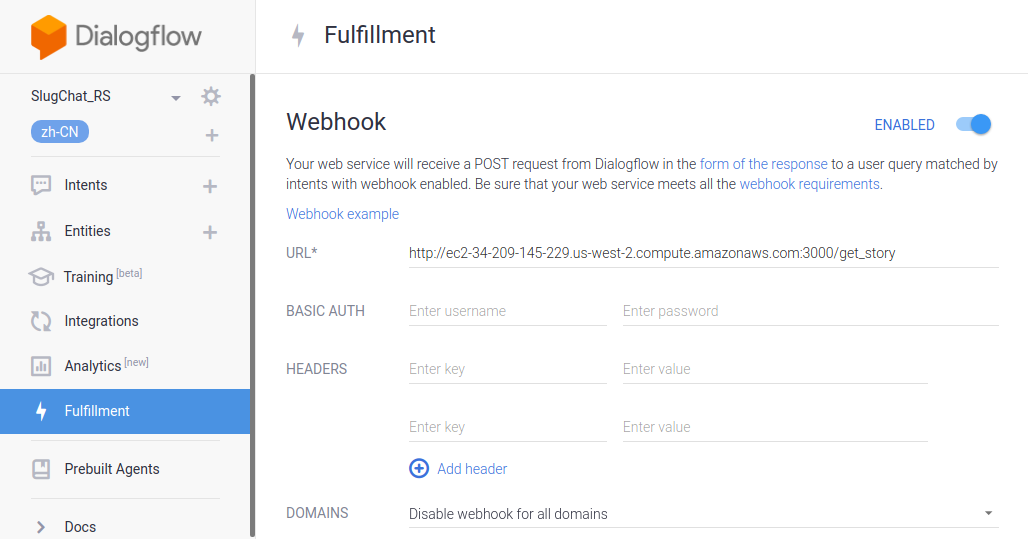
\includegraphics[width = .45\textwidth]{create_webhook.png}
\caption{Create Webhook in DialogFlow}
\label{fig:create_webhook}
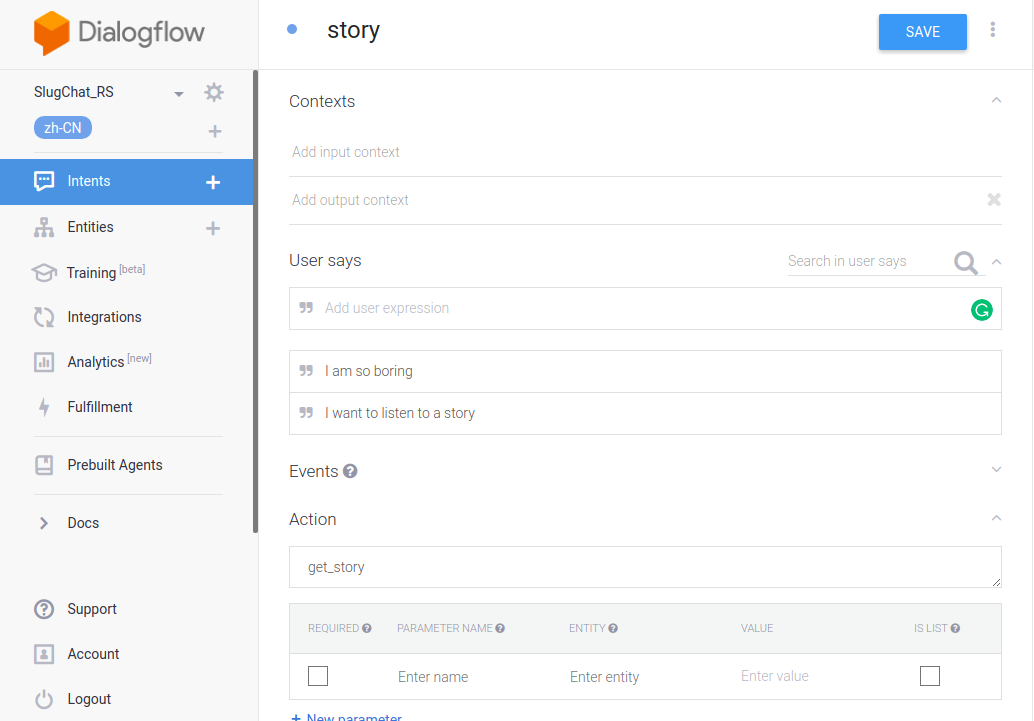
\includegraphics[width = .45\textwidth]{create_intent.png}
\caption{Create Intent in DialogFlow}
\label{fig:create_intent}
\end{figure}
\end{enumerate}
Dialogflow will send a post request to our server when a user active the webhook. This request will send a json package containing the $profileId$ of this user. When recieving this request, our server will query all logs belong to this user from $tbl\_logs$ table and get the recent listening list. Then it will return a json package with the content of a preference story to Dialogflow. At the same time, our server will write a new log into $tbl\_logs$ table.

\section{Experiments \& Disscussions}
\subsection{Word Model}
Because we don't realize the recommendation algorithm by using word2vec models. We do some experiments to test our word2vec models.
\\
Here are some tests for the performance of our models:
\begin{enumerate}
\item The most similar words to '$watermelon$' are shown in Table \ref{tab:word2vec_test}

\begin{table}
  \caption{The Top 10 Most Similar Words in Chinese to \emph{
watermelon}}
  \label{tab:word2vec_test}
  \begin{tabular}{cc}
    \toprule
    Word & Similar Coefficient\\
    \midrule
    big radish & 0.940 \\
    pear & 938 \\
    insect & 0.937 \\
    vegetables & 0.937 \\
    peach & 0.936 \\
    gourd & 0.934 \\
    nut & 0.933 \\
    candy & 0.925 \\
    shark & 0.924 \\
    carrot & 0.923 \\
  \bottomrule
\end{tabular}
\end{table}

\item The similar coefficient between '$king$' and '$princess$' is \emph{0.845}.
\item The similar coefficient between '$cock$' and '$princess$' is \emph{0.530}.
\end{enumerate}
\subsection{Recommendation Algorithm}
Then we calculate the accuracy of our LSTM model when the length of input items is 5. The accuracy of predictions is $92.1\%$. Then we separate our testing data into 2 groups by their labels. The user-like group has the accuracy with $99.4\%$ and the user-dislike group has the accuracy with $92.0\%$. It is too high to believe. 
\\\\
We change the length of input items to 6. The overall accuracy is $17.3\%$, the accuracy of the user-like group is $100\%$ and the accuracy of the user-dislike group is $17.2\%$.  We change the length of input items to 4. The overall accuracy is $99.8\%$, the accuracy of the user-like group is $5.8\%$ and the accuracy of the user-dislike group is $99.9\%$. 
\subsection{Disscussions}
The result of recommendation algorithm is really bad. We use the stable length of inputs to train the model. If we user longer inputs, it will put all inputs into the user-like group. It seems that all inputs already have 5 user-like stories and there is no need to consider whether the 6th is user-like or not. If we use shorter inputs, it will put all inputs into the user-dislike group. It seems that even the user likes the last story. No inputs in our data contain enough(5) user-like stories.

\section{Future Work}
For data part, we will use SlugChat to collect children's behaviors and use these to replace our old data.
\\
For algorithm part, we will realize the LSTM with unstable lengths of inputs and evaluate its performance. Then we will use Word Mover's Distance to replace Bag of Words to generate new story vectors. Finally, we will use the state of LSTM to replace story vectors.
\\
For SlugChat, we will replace reading stories from a text by an audio. We will also add cold start function before reading stories in order to collect users' information.

\begin{figure*}
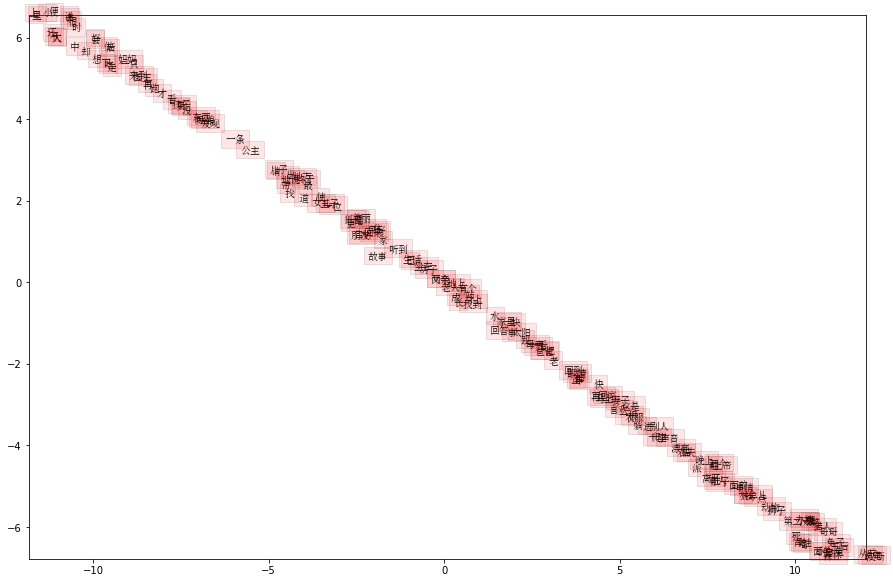
\includegraphics[width = .8\textwidth]{word2vec_1_100.png}
\caption{Word2Vec Model Distribution with Small Corpus $min \_count=1, size=100$}
\label{fig:word2vec_1_100}

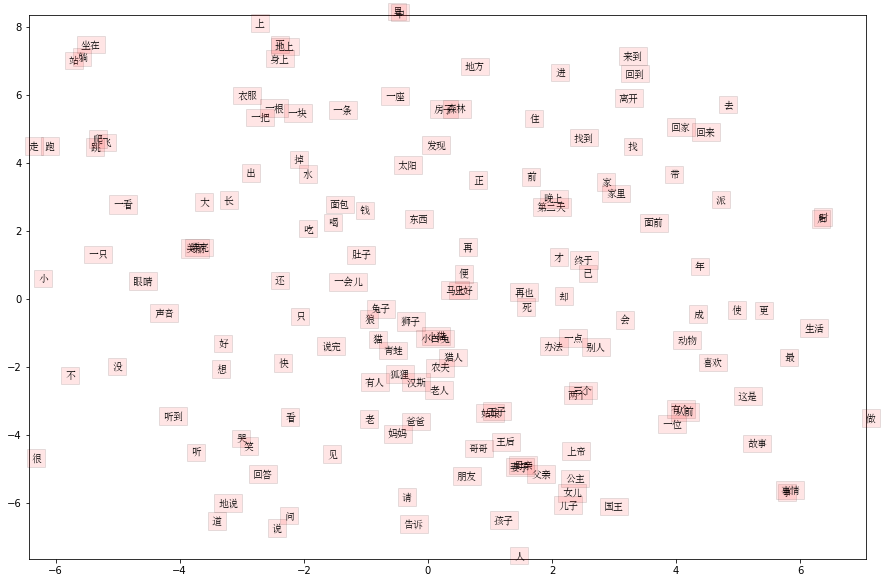
\includegraphics[width = .8\textwidth]{word2vec_15_50.png}
\caption{Word2Vec Model Distribution with Small Corpus $min \_count=1, size=50$}
\label{fig:word2vec_15_50}

\end{figure*}

\begin{figure*}
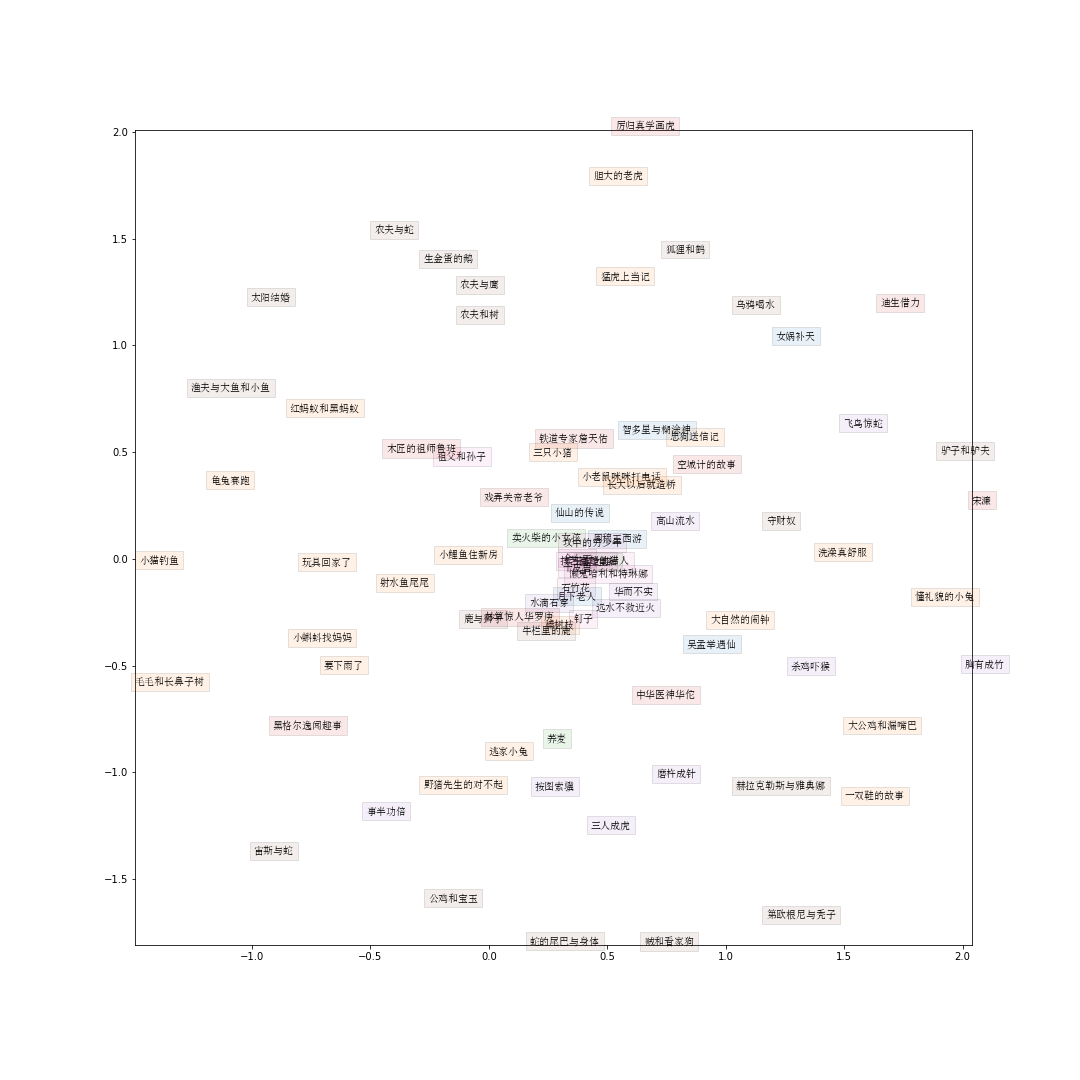
\includegraphics[width = 1.\textwidth]{story_vec.png}
\caption{BOW Story Vector Distribution}
\label{fig:story_vec}
\end{figure*}

%----------------------------------------------------------------------------------------
%	REFERENCE LIST
%----------------------------------------------------------------------------------------
\bibliography{reference}
\bibliographystyle{plain}

%----------------------------------------------------------------------------------------


\end{document}
